

\documentclass[onecolumn, draftclsnofoot,10pt, compsoc]{IEEEtran}
\usepackage{graphicx}
\usepackage{url}
\usepackage{setspace}
\usepackage{graphicx}
\usepackage{hyperref}
\usepackage{float}
\usepackage{caption}
\usepackage{subcaption}
\usepackage{minted}

% Team-added packages %%%%%%%%%%%%%%%%%%%%
\usepackage{textcomp}
%%%%%%%%%%%%%%%%%%%%%%%%%%%%%%%%%%%%%%%%%%

\usepackage{geometry}
\geometry{textheight=9.5in, textwidth=7in}

% 1. Fill in these details
\def \CapstoneTeamName{		Team Oceanographic Avoidance}
\def \CapstoneTeamNumber{		46}
\def \GroupMemberOne{			Christopher Patenaude}
\def \GroupMemberTwo{			Donald (Max) Harkins}
\def \GroupMemberThree{			Gregory Sanchez}
\def \GroupMemberFive{			Michael Gabriel}
\def \GroupMemberSix{			Tobias Hodges}
\def \CapstoneProjectName{		Self-Driving Ocean Research Vessels to Measure Glacier Retreat}
\def \CapstoneSponsorCompany{	ROSS: the Robotic Oceanographic Surface Sampler}
\def \CapstoneSponsorPerson{		Jonathan Nash}

% 2. Uncomment the appropriate line below so that the document type works
\def \DocType{	
				%Requirements Document
				%Technology Review
				%Design Document
				%Progress Report
				End-Of-Term Report
				}
			
\newcommand{\NameSigPair}[1]{\par
\makebox[2.75in][r]{#1} \hfil 	\makebox[3.25in]{\makebox[2.25in]{\hrulefill} \hfill		\makebox[.75in]{\hrulefill}}
\par\vspace{-12pt} \textit{\tiny\noindent
\makebox[2.75in]{} \hfil		\makebox[3.25in]{\makebox[2.25in][r]{Signature} \hfill	\makebox[.75in][r]{Date}}}}
% 3. If the document is not to be signed, uncomment the RENEWcommand below
%\renewcommand{\NameSigPair}[1]{#1}

%%%%%%%%%%%%%%%%%%%%%%%%%%%%%%%%%%%%%%
% https://tex.stackexchange.com/questions/322196/how-to-cite-a-url-in-ieeetran-bib-file

\usepackage{filecontents}
\begin{filecontents*}{\jobname.bib}
@MISC{wiki,
  author = {Wikipedia},
  title  = {Pairing function {@MISC}},
  month  = May,
  year   = {2016},
  url    = {https://en.wikipedia.org/wiki/Pairing_function/},
}
@MISC{dlib-interface,
  title  = {Dlib Python API},
  month  = Sep,
  year   = {2019},
  url    = {http://dlib.net/python/index.html},
}
@MISC{dlib,
  title  = {Dlib C++ Library},
  month  = Sep,
  year   = {2019},
  url    = {http://dlib.net/},
}
@MISC{vlfeat,
  title  = {vlfeat},
  organization = {Github},
  month  = Jan,
  year   = {2018},
  url    = {https://github.com/vlfeat/vlfeat},
}
@MISC{opencv-about,
  title  = {About},
  organization = {OpenCV},
  url    = {https://opencv.org/about/},
}
@MISC{opencv-intro,
  title  = {OpenCV 2.4.13.7 documentation - Introduction},
  organization = {OpenCV},
  month  = Nov,
  year   = {2019},
  url    = {https://docs.opencv.org/2.4/modules/core/doc/intro.html},
}
@MISC{opencv-python,
  title  = {Introduction to OpenCV-Python Tutorials},
  organization = {OpenCV},
  month  = Nov 10,
  year   = {2014},
  url    = {https://docs.opencv.org/3.0-beta/doc/py_tutorials/py_setup/py_intro/py_intro.html},
}
@MISC{opencv-SIFT,
  title  = {Introduction to SIFT (Scale-Invariant Feature Transform)},
  organization = {OpenCV},
  url    = {https://opencv-python-tutroals.readthedocs.io/en/latest/py_tutorials/py_feature2d/py_sift_intro/py_sift_intro.html#sift-intro},
}
@MISC{opencv-SURF,
  title  = {Introduction to SURF (Speeded-Up Robust Features)},
  organization = {OpenCV},
  url    = {https://opencv-python-tutroals.readthedocs.io/en/latest/py_tutorials/py_feature2d/py_surf_intro/py_surf_intro.html},
}
@MISC{opencv-ORB,
  title  = {ORB (Oriented FAST and Rotated BRIEF)},
  organization = {OpenCV},
  url    = {https://opencv-python-tutroals.readthedocs.io/en/latest/py_tutorials/py_feature2d/py_orb/py_orb.html},
}
@MISC{comparison,
  author = {Shehan Akalanka Perera},
  title  = {A Comparison of SIFT , SURF and ORB},
  month  = Aug,
  year   = {2018},
  url    = {https://medium.com/@shehan.a.perera/a-comparison-of-sift-surf-and-orb-333d64bcaaea},
}
@MISC{feature-match,
  title  = {Feature Matching},
  organization = {OpenCV},
  month  = Nov,
  year   = {2019},
  url    = {https://docs.opencv.org/master/dc/dc3/tutorial_py_matcher.html},
}
@MISC{bfmatcher,
  title  = {cv::BFMatcher Class Reference
},
  organization = {OpenCV},
  month  = Nov,
  year   = {2019},
  url    = {https://docs.opencv.org/3.4/d3/da1/classcv_1_1BFMatcher.html},
}
@MISC{flann-user-man,
  title  = {FLANN - Fast Library for Approximate Nearest Neighbors},
  author = {Marius Muja and David Lowe},
  type = "manual",
  month  = Jan,
  year   = {2013},
  url    = {https://www.cs.ubc.ca/research/flann/},
}
@MISC{pyserial,
  title  = {Docs – pySerial},
  type = "manual",
  url    = {https://pyserial.readthedocs.io/en/latest/pyserial.html},
}
@MISC{coastguard,
  title  = {U.S. Dept of Homeland Security U.S. Coast Guard, “Navigation Rules International – Inland,”},
  url    = {https://www.navcen.uscg.gov/pdf/navRules/navrules.pdf},
}

\end{filecontents*}
%%%%%%%%%%%%%%%%%%%%%%%%%%%%%%%%%%%%%%%

% Glossaries
\usepackage[utf8]{inputenc}
\usepackage[acronym,nonumberlist]{glossaries}
\setlength\LTleft{0pt}
\setlength\LTright{0pt}
\setlength\glsdescwidth{5in}
\renewcommand{\glsnamefont}[1]{\textbf{#1}}
\makeglossaries

\newacronym{aov}{AOV}{Autonomous Ocean Vessel}
\newacronym{ross}{ROSS}{Robotic Oceanographic Surface Sampler}
\newacronym{gpu}{GPU}{Graphics Processing Unit}
\newacronym{cpu}{CPU}{Central Processing Unit}
\newacronym{lan}{LAN}{Local Area Network}
\newacronym{usv}{USV}{Unmanned Surface Vessel}
\newacronym{gps}{GPS}{Global Positioning System}
\newacronym{oas}{OAS}{Object Avoidance System}
\newacronym{nuc}{NUC}{Next Unit of Computing: Intel® Mini-computers}
\newacronym{orb}{ORB}{Oriented FAST (Features from Accelerated and Segments Test) and Rotated BRIEF (Binary Rough Independent Elementary Feature): Feature detection and description algorithm developed at OpenCV labs}
\newacronym{flann}{FLANN}{Fast Library for Approximate Nearest Neighbors: library containing a collection of algorithms optimized for fast nearest neighbor search}
\newacronym{colregs}{COLREGS}{Convention on the International Regulations for Preventing Collisions at Sea}
\newacronym{smd}{SMD}{Singapore Maritime Dataset}


%%%%%%%%%%%%%%%%%%%%%%%%%%%%%%%%%%%%%%

\begin{document}
\begin{titlepage}
    \pagenumbering{gobble}
    \begin{singlespace}
    	%\includegraphics[height=4cm]{coe_v_spot1}
        \hfill 
        % 4. If you have a logo, use this includegraphics command to put it on the coversheet.
        %\includegraphics[height=4cm]{CompanyLogo}   
        \par\vspace{.2in}
        \centering
        \scshape{
            \huge CS Capstone \DocType \par
            {\large\today}\par
            \vspace{.5in}
            \textbf{\Huge\CapstoneProjectName}\par
            \vfill
            {\large Prepared for}\par
            \Huge \CapstoneSponsorCompany\par
            \vspace{5pt}
            {\Large\NameSigPair{\CapstoneSponsorPerson}\par}
            {\large Prepared by }\par
            Group\CapstoneTeamNumber\par
            % 5. comment out the line below this one if you do not wish to name your team
            \CapstoneTeamName\par 
            \vspace{5pt}
            {\Large
                \NameSigPair{\GroupMemberOne}\par
                \NameSigPair{\GroupMemberTwo}\par
                \NameSigPair{\GroupMemberThree}\par
                \NameSigPair{\GroupMemberFour}\par
                \NameSigPair{\GroupMemberFive}\par
                \NameSigPair{\GroupMemberSix}\par
            }
            \vspace{20pt}
        }
        \begin{abstract}
        % 6. Fill in your abstract   
This document describes the current state of the Autonomous Vessel Vision System (AVVS) being implemented for the Robotic Oceanographic Surface Sampler (ROSS). The AVVS is intended to provide environmental awareness to ROSS via monocular computer vision and a pre-trained neural network which persistently tracks objects, like boats, in front of the ROSS. The components of the AVVS are each individually functional and pass eyeball testing. Over the course of Spring term, we will be integrating the AVVS into the ROSS begin more rigorous testing: unit, and environmental testing.

        \end{abstract}     
    \end{singlespace}
\end{titlepage}
\newpage
\pagenumbering{arabic}
\tableofcontents
% 7. uncomment this (if applicable). Consider adding a page break.
%\listoffigures
%\listoftables
\clearpage

% 8. now you write!
\section{Introduction}

% Subsequent 2 sections copied from last term's progress report (with some modifications)
\subsection{Project Purpose}
The system our team (Capstone Team 46) is building is intended to let an autonomous marine surface vessel detect and report obstacles in the water. The system is  intended for use on a small, 12 ft inflatable vessel equipped for oceanographic research. With a sufficiently sophisticated object avoidance system, a research USV would be able to operate for extended periods of time without direct supervision, allowing for the collection of valuable oceanographic data. Intended uses for our system include research trips to the Gulf of Mexico and Alaska. The use of our system would facilitate collection of data that would inform scientists about ocean processes such as glacial melt at ocean-glacier interfaces. Our system would reduce the potential for collisions between an autonomous research vessel the system is deployed on, and floating debris or other vessels.



\subsection{Project Goals}
Goals of this project are to implement an obstacle detection module to detect obstacles from video of the environment, interface the modules with the preexisting navigation and communication systems on board the research vessel, persistently track detected objects over time, and report the relative position of detected obstacles in real time to an external system. At the end of the Capstone project, it is desired that our system can detect more than 90\% of the objects it encounters in average operating conditions, with minimum false positives.


\section{Current Status}
Our system includes four main software components. These are an image processing module, obstacle classifier/detector, persistent object tracker, and an object position reporting module. Additionally, to support the image processing and object reporting components, we use an additional IMU (Inertial Measurement Unit) data collection module, which collects positional data for the boat needed for the other components to function.

%LaTeX has a really annoying feature of not fixing the position of a figure on the page to it's position in the .tex doc 
\begin{figure}[H]
\centering
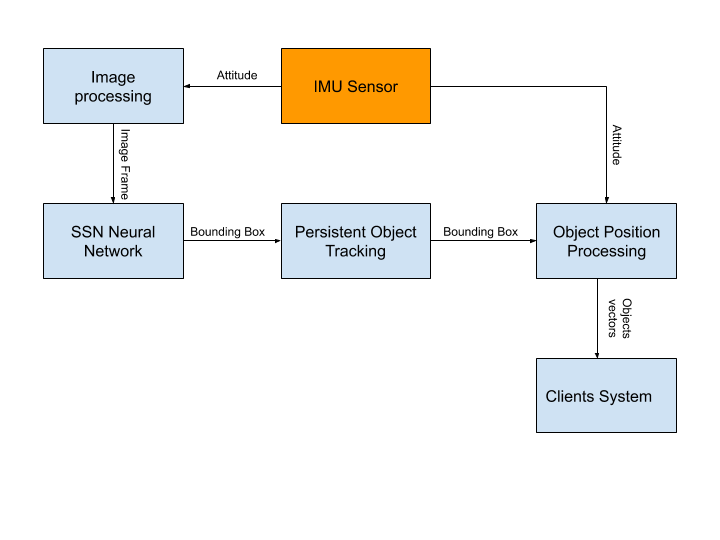
\includegraphics[width=0.9\textwidth]{./Planz.png}
\caption{Autonomous Vessel Vision System software component interaction}
\label{fig:componentDiagram}
\end{figure}

\subsection{Problems Encountered}
The design of our system and the goals of our project changed over the last term. 
%\subsubsection{Stereo Vision and Depth Mapping}
%From Tobias' stereo vision slide
A major challenge for our project was to implement a stereo camera system to determine the distances to any detected objects. This was to be a major component of our system, and central to determining the exact positions of objects detected. We chose stereo vision as a method of determining depth because of the low cost, relatively large theoretical distance for accurate depth determination, and the ability to generate depth maps for large fields of view. However, we had difficulty implementing a stereo vision system in non-stationary environments. We had some success with very stable stereo cameras in a testing environment, but out on the open waters, the system has to be just as reliable, and we were not able to accomplish this. Stereo vision also posed some issues when attempting to deserialize and synchronize the data from two separate cameras into usable information. There were options on the market for camera systems built for this purpose, where two attached cameras would produce synchronized data, even some products that included a processing unit to output depth maps automatically, but all the issues we were running into made us question if we had really made the right choice with stereo vision in the first place. This conversation led to the group reevaluating almost everything that we were attempting to do, and brought up the question of what the most valuable kind of data would be for a navigation system.

We looked into many different solutions, and even considered some products that produced ready-made depth maps, but after a lot of research and discussion, we decided that we wanted to focus more on continuous object recognition and reporting. We also decided that the actual distance mapping was a lot less valuable than determining where objects were in direct relation to the vessel and the intended path of navigation. In other words: if the vessel is traveling forward in a straight line at a specific angle, where are the obstacles relative to the angle of travel? We came up with a system that tracks objects with computer vision and relays that data to an operator, all while accounting for the conditions that the vessel would face on the open water.

\subsection{IMU Data Collection Status}
The Inertial Measurement Unit (IMU) is a hardware component of the ROSS USV which our project utilizes to collect attitude data on the current orientation of the USV in space. The IMU transmits a constant stream of serialized data packets at 10Hz to our clients system where it is written to a file for easy access. The AVVS's IMU module interfaces with a 3ed party MatLab script (provided by clients) to parse serial data from the IMU data file into a python dictionary following the structure described in figure \ref{fig:IMUDataStruct}. The IMU module can be called, by other AVVS modules, to retrieve the ROSS's most recent attitude to compensate for USV position. The IMU module is currently functional and has been tested with real data collected from the ROSS's data logs. The IMU was implemented with a python class and should be very easily usable by any of the AVVS's other components. All functions in the IMU class are currently unit tested.

\begin{figure}[H]
\begin{minted}[frame=lines,
               framesep=2mm,
               linenos=false,
               xleftmargin=21pt,
               tabsize=4]{js}
'units': {
    'attitude': { 
        'compensated_angular_rate': { 
            'X': 'rads/sec',
            'Y': 'rads/sec',
            'Z': 'rads/sec',
            'valid': '1=valid, 0=invalid'
        },
        'gps_timestamp': { 
            'time_of_week': 'seconds',
            'valid': '1=valid, 0=invalid',
            'week_number': 'n/a'
        },
        'heading_update_source_state': { 
            'heading': 'radians',
            'heading_1_sigma_uncertainty': 'radians',
            'source': '0=no source, 1=Magnetometer, 4=External',
            'valid': '1=valid, 0=invalid'
        },
        'linear_acceleration': { 
            'X': 'm/sec^2',
            'Y': 'm/sec^2',
            'Z': 'm/sec^2',
            'valid': '1=valid, 0=invalid'
        },
        'orientation_euler_angles': { 
            'pitch': 'radians',
            'roll': 'radians',
            'valid': '1=valid, 0=invalid',
            'yaw': 'radians'
        }
    }
}
\end{minted}
\caption{IMU attitude data format} 
\label{fig:IMUDataStruct}
\end{figure}

\subsection{Image Processing Status}

As the vessel is moving through open waters, the frame by frame input we gather from the video feed has differentiating images. Each frame will be altered by the ocean waves. One frame may be tilted by the USV's roll, or another frame may be tilted by the USV's pitch. The differences in each frame will be significant enough to effect the persistent object tracking status later described in \hyperref[sec:2.5]{2.5}. To account for this, we can use the IMU positional data to transform the image. 

With the IMU positional data, we can use the Euler angles (pitch, roll and yaw) to transform each image so that they are on the same level of horizon. To do this we can use matrices multiplication from the Euler angles to obtain a rotation matrix. We can also formulate a camera calibration intrinsic matrix from the specifications (focal length/sensor width) with the camera we used. After this we then create a final transformation matrix that multiplies all of these matrices together. Then, the final transformation matrix can  be used on the image we are processing to then transform the image from the IMU positional data. An example transformation from an about 30\textdegree  roll can be seen in \hyperref[fig:image-processing]{figure below}

\begin{figure}[H]
\centering
\begin{subfigure}{.5\textwidth}
  \centering
  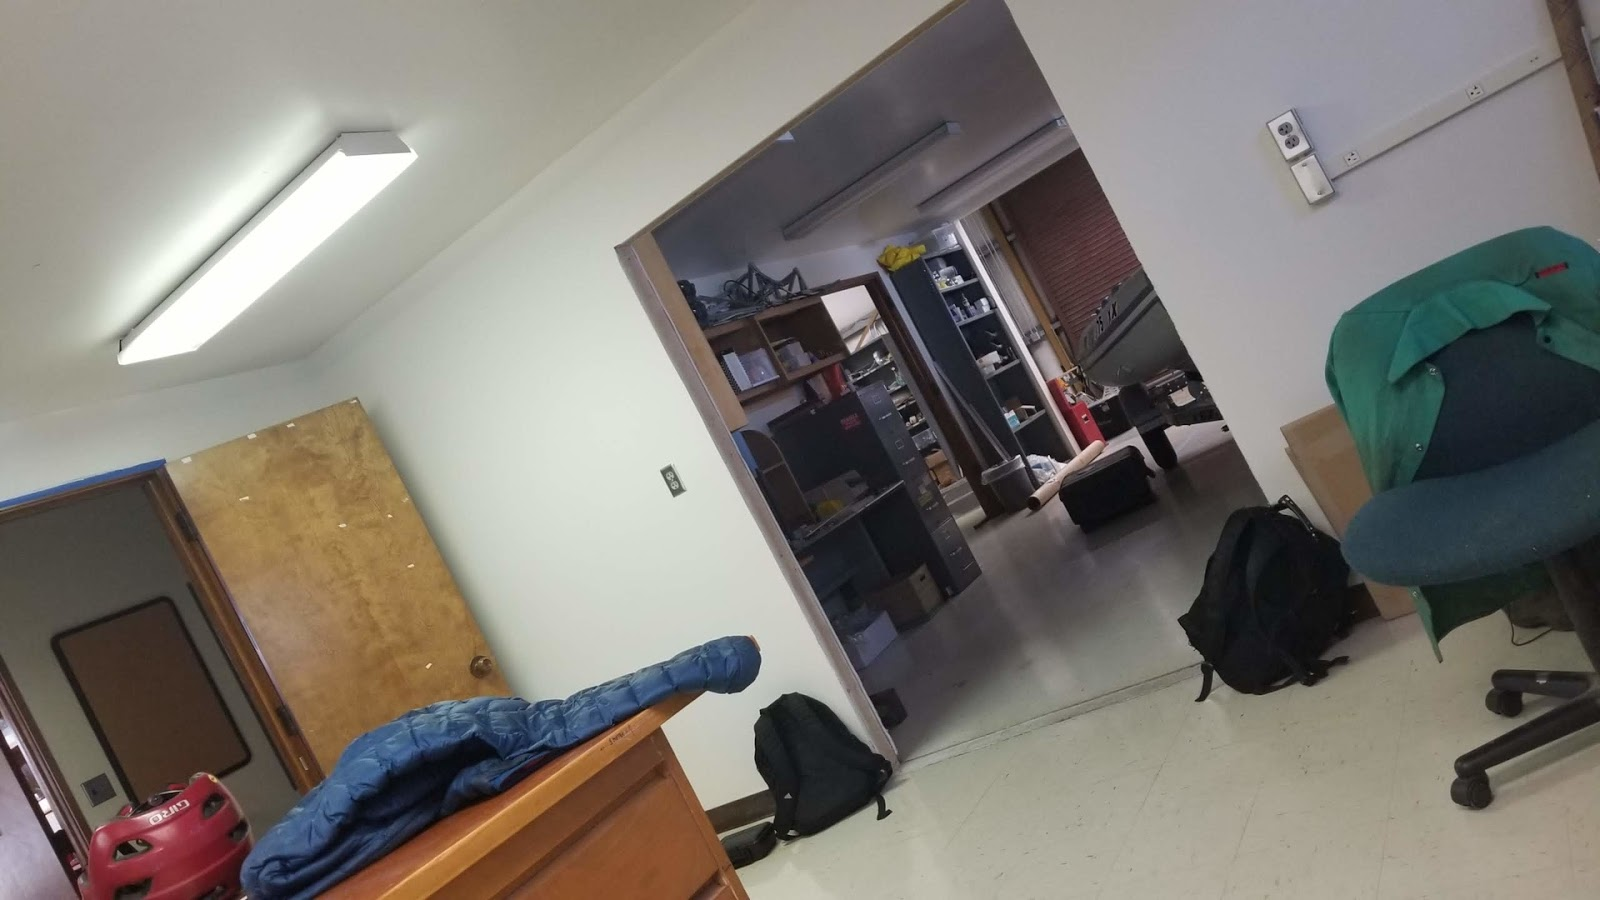
\includegraphics[width=3in]{cs462_img_proc_before.jpg}
  \caption{Example unaltered input frame  (skewed roll by $\sim$30\textdegree)}
  \label{fig:sub1}
\end{subfigure}%
\begin{subfigure}{.5\textwidth}
  \centering
  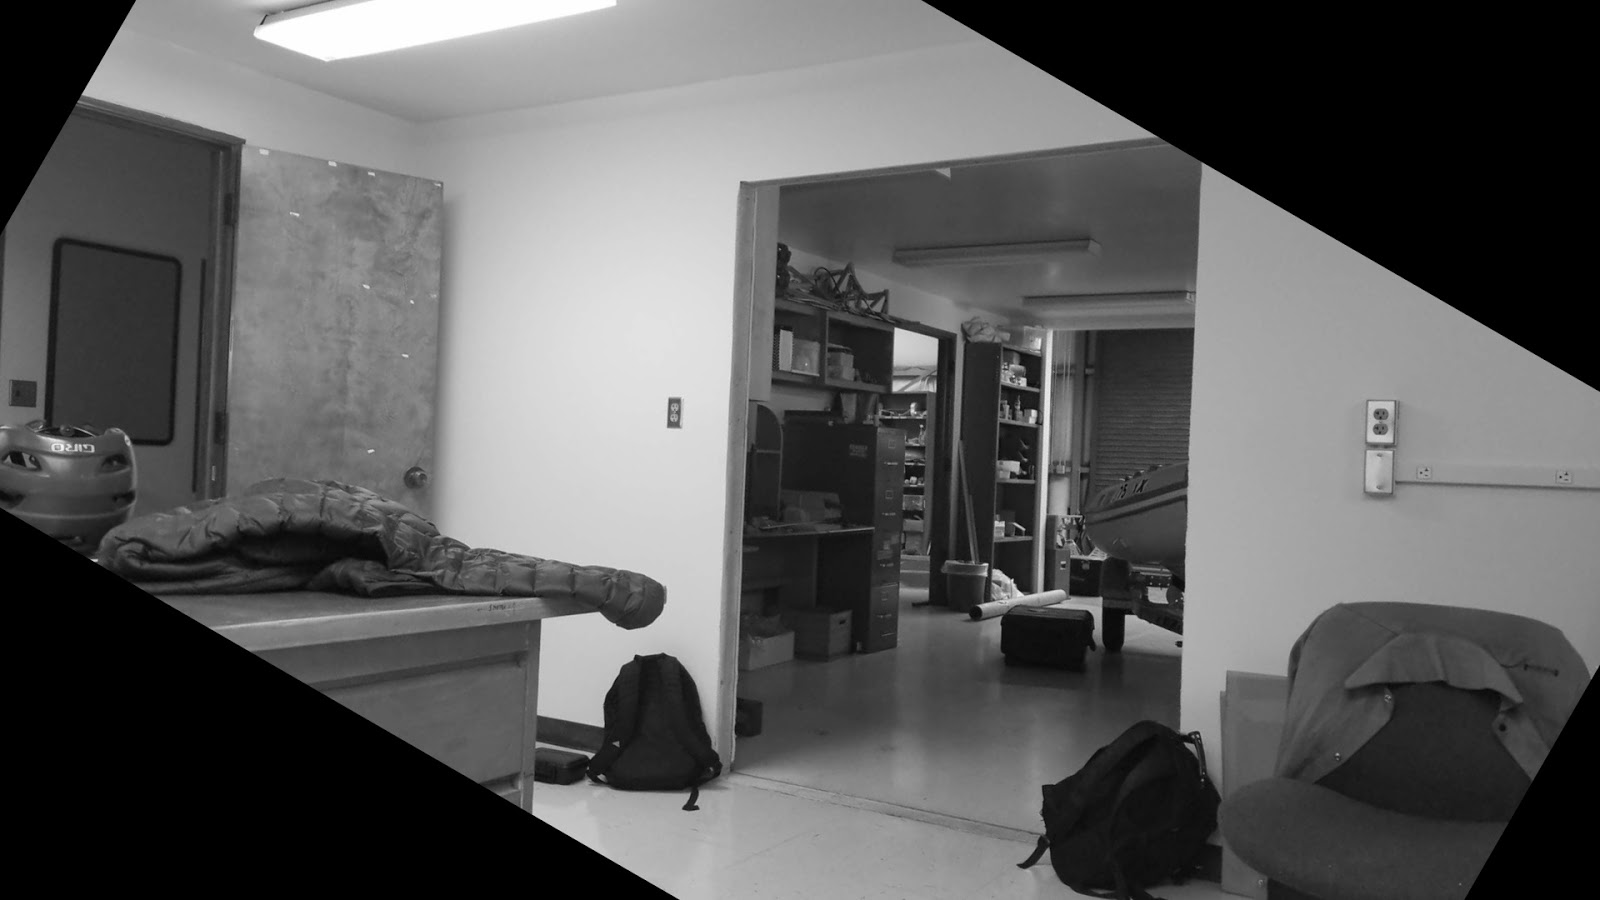
\includegraphics[width=3in]{cs462_img_proc_after.jpg}
  \caption{Transformed Image }
  \label{fig:sub2}
\end{subfigure}
\caption{Image Processing Example}
\label{fig:image-processing}
\end{figure}

\subsection{Obstacle Classifier Status}
After being captured from the on-board camera and processed by the image processing module, images will be fed into the obstacle classification module. The obstacle classification module uses a deep neural network to detect and classify any objects present in the image. Using a deep (convolutional) neural network, our system is able to determine with confidence the rectangular regions in an image where obstacles exist, in real time. The specific neural network we chose to use was a Single Shot Detector with Inception V2 architecture. This neural network is rapid and accurate at determining where and what obstacles are present in an image. It takes as input a scaled image 300 by 300 pixels in dimension, and outputs an list of detected objects, each object having a confidence percentage, a label of the object type, and a pair of coordinates representing the position of a rectangular 'box' within the input image. On an i7 laptop processor, our current system is able to run at approximately fifteen frames per second. While the on board navigation computer of the autonomous vessel, where we will ultimately install the system, uses a less-powerful Intel i3 processor, we anticipate our system will still operate in near real time, producing one or more frames per second. Our client finds this speed acceptable given the low-performance nature of the system, and limited power available for operation.

Neural networks are able to detect and classify objects only after being trained on an extensive set of data. The SSD Inception network we are using was trained on the Singapore Maritime Dataset (SMD), 
% https://sites.google.com/site/dilipprasad/home/singapore-maritime-dataset
which consists of hundreds of annotated images of boats and other marine objects  taken in the ocean near Singapore. From training on the SMD, our neural network is able to recognize various ocean vessels (sailboats, speedboats, ships, ferries, kayaks, generic boats), buoys, swimming people, and airplanes/flying objects. Images in the SMD consist of pictures of ocean with minimal other scenery. Thus, the neural network produces the least false positives in similar environments where there is little observable land with scenery other than waves. The environment of the Gulf of Mexico, where the system will be used this summer, will closely resemble the environment used for training. 

One shortcoming of the neural network used is that it has not been trained on floating ice or obstacles present in an arctic environment. Re-training a neural network is non-trivial, and our team does not have a dataset of floating sea ice obstacles that could be used for training. Hence, we have decided to focus on building a system that primarily detects and reports other vessels and people.

\subsection{Persistent Object Tracking Status}
\label{sec:2.5}
The neural network object detector/classifier only reports objects found in individual frames, and has no way to persistently track objects between frames. Hence, a persistent object tracking module is used to associate bounding boxes between images, and identify and track objects over time. The object tracker works by minimizing the euclidean distances between the centers, called centroids, of bounding boxes found in the most recently captured image and the previously determined bounding boxes.

The general algorithm for the centroid tracker is as follows:
\begin{itemize}
    \item For $n$ objects found in the current frame and $m$ objects being tracked by the detector, initialize an $n \times m$ matrix (or other data structure) to store the distances between centroids. 
    
    \item For each object $i$ in the current frame, compute the distance between the center point of the bounding box containing it and the center points for every object in the previous image using the L2 norm. Store these values in the $i$'th row of the distance matrix.
    
    \item After the matrix has been filled, for each row, find the minimum distance in the row. Store these values in a new vector (or list) of size $n$. 
    
    \item Next, sort the vector of minimum row values from least to greatest.
    
    \item While there are objects being tracked that remain disassociated with an object in the new frame, iterate through the sorted vector. For each entry, determine the corresponding column and row indices in the original matrix. Associate the objects corresponding to the row and column from the original matrix, and mark the object from the previously tracked objects as associated.
    
    \item If there are more objects in the new image than the previous, add the rest of the objects as new objects to the tracking system.
    
    \item If there are fewer objects in the new image than are being tracked, mark the extra objects as being out of frame. If an object has been out of frame for more than 10 frames, remove it from the tracker.
\end{itemize}
Because this algorithm only matches the centers of bounding boxes, and does not use information about the size of the bounding boxes, it is inaccurate for situations where there are many objects of different sizes clustered together. However, since the described situation is unlikely to occur in a marine environment, the algorithm is sufficient. Additionally, ignoring the size of the bounding box and treating each object as a single point makes the algorithm more efficient and slightly faster.

Having a persistent tracking algorithm allows us to track data about the detected objects over time. Along with the previously known centroid position for each obstacle, when an obstacle is detected in an image a data object is added to a list associated with the detected object. For each detection, the list stores the timestamp.

\subsection{Object Position Reporting Status}
The Object Position Reporting module of our project receives necessary data from the Obstacle Classifier and Persistent Object Tracking Modules to determine the required pixels needed to find the angle of the object from the heading of the research vessel. The module also requires the height and width of the picture in pixels as well as the number of degrees the view port of the visual sensor—in our case, a Logitech web camera. This function will work by finding the angle each pixel in an image will represent. To find this number we have to divide the length of the image diagonal in pixels by the number of degrees that the camera view port has on the same diagonal. For example a camera with a view port of forty-five degrees that captures 1280 by 720 pixels will have roughly 0.031 degrees per pixel from the center of the image. To find the angle of an object from the center of the view port we need to find the distance from the center and multiply it by the scalar.

\section{Plans for Spring Term}

\subsection{Client Integration}
For spring term, the team will work on integrating the object detection system with the client user interface. This will allow the user to see the headings of other objects in relation to the ROSS' vector of navigation. Upon integrating the object detection system with the client interface, the system will be fully testable and will undergo repeated autonomous tests.

\subsection{Testing}
After completion of the base object detection system, the ROSS will be taken onto open waters and presented with a series of test obstacles from which we will be able to take data and compare it to expected values on the client interface. Once the system is determined to properly detect the test objects, the ROSS will be taken on a series of local test runs. After test runs are deemed successful, the ROSS will execute a mission utilizing the object detection system.

\end{document}
